% trap_ranuras. GENERADO por figuras_recuperacion.py: no editar a mano.
\documentclass[border=0pt,tikz]{standalone}
\usepackage[utf8]{inputenc}
\usepackage[T1]{fontenc}
\usepackage{lmodern}
\usepackage[none]{hyphenat}
% Estilo común de las figuras TikZ (panoramas y diagramas de bloques).
%
% Cada figura lo incluye con \input{../../figuras/estilo_tikz.tex} (las figuras
% viven en docs/<módulo>/figuras/). Un solo lugar para la paleta, los estilos de
% bloque y el formato de los parámetros: si cambia algo acá, cambia en todas.
%
% La paleta es la misma de docs/figuras/estilo_svg.py y de PALETA en
% modulos/mk/datasheet.py; si se toca un color, se toca en los tres.
%
% Requiere: \usepackage{tikz} (lo da la clase standalone con la opción tikz).

\usetikzlibrary{arrows.meta,positioning,calc,fit,backgrounds,shapes.multipart,
                decorations.markings,shadows}

% ---------------------------------------------------------------- colores ---
\definecolor{azul}{RGB}{108,172,228}      % acondicionamiento
\definecolor{verde}{RGB}{110,214,142}     % captura / histogramas en BRAM
\definecolor{amarillo}{RGB}{252,232,160}  % trigger
\definecolor{naranja}{RGB}{252,206,160}   % camino a DDR
\definecolor{grisr}{RGB}{226,226,226}     % compartido / infraestructura
\definecolor{rojo}{RGB}{240,128,128}      % bus del sistema

% ---------------------------------------------------------------- estilos ---
\tikzset{
  >={Stealth[length=2.4mm,width=1.8mm]},
  % fondo blanco siempre: el SVG se ve igual en modo claro y oscuro
  fondo/.style   = {show background rectangle, inner frame sep=8pt,
                    background rectangle/.style={fill=white, draw=none}},
  bloque/.style  = {draw=black, line width=0.6pt, rounded corners=2pt,
                    align=center, text width=2.2cm, minimum height=1.15cm,
                    inner sep=2pt, font=\scriptsize, fill=#1},
  datos/.style   = {bloque=azul!35},
  trig/.style    = {bloque=amarillo},
  captura/.style = {bloque=verde!55},
  ddr/.style     = {bloque=naranja!70},
  comp/.style    = {bloque=grisr},
  bus/.style     = {bloque=rojo!45},
  % lógica escrita dentro del módulo, sin submódulo propio
  etapa/.style   = {bloque=#1, line width=0.5pt},
  etapa/.default = verde!20,
  % lo que el bitstream no trae (atado a cero, stub, salida muda)
  mudo/.style    = {bloque=white, draw=black!45, dashed, text=black!55},
  %
  % BLOQUE CON PARÁMETROS, en el formato del datasheet: el encabezado lleva el
  % nombre y los parámetros con que lo instancia el padre (NOMBRE=valor, en
  % monoespaciada, uno por línea); el cuerpo, más claro, lo que hace.
  %   \node[datos, param={azul!35}{azul!12}] {\blk{nombre}{} \prm{A=1\\B=2}
  %                                            \nodepart{two} función};
  param/.style 2 args = {rectangle split, rectangle split parts=2,
                         rectangle split part fill={#1, #2}},
  %
  flujo/.style   = {->, line width=0.8pt},
  ctrl/.style    = {->, line width=0.6pt, black!65},
  % la línea que pasa por encima en un cruce: un halo blanco la separa
  cruce/.style   = {preaction={draw=white, line width=3.4pt, -}},
  % marca de ancho de bus: barra oblicua a mitad de la flecha, con el número
  % encima. \draw[flujo, ancho=14] ...; para otra posición, ancho en=0.3.
  ancho/.style   = {decoration={markings, mark=at position \anchopos with {
                      \draw[line width=0.6pt, -] (-0.1,-0.14) -- (0.1,0.14);
                      \node[font=\scriptsize, above=1.5pt] {#1};}},
                    postaction={decorate}},
  % la misma marca en una flecha vertical: el número va a la derecha
  anchov/.style  = {decoration={markings, mark=at position \anchopos with {
                      \draw[line width=0.6pt, -] (-0.14,-0.1) -- (0.14,0.1);
                      \node[font=\scriptsize, right=3pt] {#1};}},
                    postaction={decorate}},
  ancho en/.code = {\def\anchopos{#1}},
  sen/.style     = {font=\scriptsize\ttfamily, inner sep=1.5pt},
  nodo/.style    = {font=\tiny\ttfamily, inner sep=1pt, black!75},
  pin/.style     = {font=\scriptsize, align=center, inner sep=1pt},
  grupo/.style   = {draw=black!55, dashed, line width=0.7pt, rounded corners=4pt},
  canal/.style   = {grupo},
  contenedor/.style = {draw=black!80, line width=1.0pt, rounded corners=6pt},
  % marca numerada: cada número es una fila de la tabla del documento
  marca/.style   = {circle, fill=black, text=white, font=\scriptsize\bfseries,
                    inner sep=0pt, minimum size=4.3mm},
  %
  % DECISIONES (docs/mca/vista_general_mca.md). Cada opción es un bloque, todas
  % entran a un mux (\muxdec, abajo) y el registro que elige entra por abajo.
  % la opción que trae el reset (el comportamiento histórico): borde doble
  defecto/.style = {double=white, double distance=0.8pt, line width=0.45pt},
  % rótulo de la decisión, el mismo Dn del panorama y del documento
  decision/.style = {circle, fill=black, text=white, font=\small\bfseries,
                     inner sep=0pt, minimum size=7mm},
  %
  % LÓGICA (docs/mca/figuras/contabilidad/ y los detalles de las decisiones)
  % registro: caja gris con el triángulo de reloj en el borde de abajo
  registro/.style = {draw=black, line width=0.6pt, fill=grisr, align=center,
                     font=\scriptsize, inner sep=2pt, minimum width=#1,
                     minimum height=0.85cm,
                     path picture={\draw[line width=0.5pt]
                       ([xshift=-1.1mm]path picture bounding box.south) --
                       ([yshift=1.6mm]path picture bounding box.south) --
                       ([xshift=1.1mm]path picture bounding box.south);}},
  registro/.default = 0.8cm,
  % condición de una cadena if / else-if: "sí" sale a la derecha, "no" abajo
  pregunta/.style = {draw=black, line width=0.5pt, rounded corners=7pt,
                     fill=white, font=\scriptsize\ttfamily, align=center,
                     inner sep=2.5pt, minimum height=0.62cm, text width=#1},
  pregunta/.default = 1.9cm,
  si/.style      = {font=\tiny, inner sep=1pt, above, pos=0.12},
  no/.style      = {font=\tiny, inner sep=1pt, left, pos=0.45},
  %
  titulo/.style  = {anchor=north west, font=\small, inner sep=4pt, align=left},
  rotulo/.style  = {anchor=north west, font=\scriptsize\itshape, black!70,
                    inner sep=2pt, align=left},
}

% submódulo: nombre en monoespaciada; lógica propia: nombre en romana
\newcommand{\blk}[2]{{\ttfamily\bfseries #1}\\[1pt]#2}
\newcommand{\etq}[2]{{\bfseries #1}\\[1pt]#2}
\newcommand{\punto}[1]{\fill (#1) circle (1.3pt);}

% Parámetros en el formato del datasheet: NOMBRE=valor en monoespaciada, una
% entrada por celda, hasta cuatro columnas. Una columna: \prm{A=1\\B=2};
% dos: \prm{A=1 & B=2\\C=3}.
\newcommand{\prm}[1]{{\ttfamily\fontsize{5.6}{6.6}\selectfont
  \begin{tabular}{@{}l@{\hspace{7pt}}l@{\hspace{7pt}}l@{\hspace{7pt}}l@{}}#1\end{tabular}}}

\def\anchopos{0.5}

% Mux de una decisión: trapecio con el lado ancho (las entradas) a la izquierda.
% #1 = nombre, #2 = centro, #3 = alto en cm. Deja tres coordenadas:
%   (#1-in)  centro del lado de entradas: las flechas llegan a (#1-in |- opcion.east)
%   (#1-out) la salida
%   (#1-sel) mitad del lado de abajo: por ahí entra el registro que elige
% El rótulo de adentro es opcional: \muxdec{m}{(4,0)}{3.6} y después
% \node[...] at (m) {...}.
\newcommand{\muxdec}[3]{%
  \path #2 coordinate (#1);
  \draw[line width=0.6pt, fill=grisr]
    ($(#1)+(-0.45,{#3/2})$) -- ($(#1)+(0.45,{#3/2-0.35})$) --
    ($(#1)+(0.45,{-#3/2+0.35})$) -- ($(#1)+(-0.45,{-#3/2})$) -- cycle;
  \coordinate (#1-in)  at ($(#1)+(-0.45,0)$);
  \coordinate (#1-out) at ($(#1)+(0.45,0)$);
  \coordinate (#1-sel) at ($(#1)+(0,{-#3/2+0.175})$);}

% El mismo mux rotado 90 grados, para un flujo de arriba hacia abajo: entradas
% por el lado ancho de arriba, salida abajo y el registro que elige por la
% izquierda. #1 = nombre, #2 = centro, #3 = ancho en cm. Deja (#1-in) centro del
% lado de entradas, (#1-out) la salida y (#1-sel) mitad del lado izquierdo.
\newcommand{\muxdecv}[3]{%
  \path #2 coordinate (#1);
  \draw[line width=0.6pt, fill=grisr]
    ($(#1)+({-#3/2},0.45)$) -- ($(#1)+({#3/2},0.45)$) --
    ($(#1)+({#3/2-0.35},-0.45)$) -- ($(#1)+({-#3/2+0.35},-0.45)$) -- cycle;
  \coordinate (#1-in)  at ($(#1)+(0,0.45)$);
  \coordinate (#1-out) at ($(#1)+(0,-0.45)$);
  \coordinate (#1-sel) at ($(#1)+({-#3/2+0.175},0)$);}

% Leyenda de colores + nota. #1 = posición, #2 = color/texto, #3 = nota.
\newcommand{\leyenda}[3]{%
  \begin{scope}[shift={(#1)}, every node/.style={font=\scriptsize}]
    \coordinate (t0) at (-0.5,0);
    \foreach \c/\t [count=\i] in {#2} {
      \pgfmathtruncatemacro\j{\i-1}
      \node[draw, fill=\c, minimum width=4mm, minimum height=3mm, inner sep=0pt,
            right=5mm of t\j.east, anchor=west] (l\i) {};
      \node[right=1.5mm of l\i] (t\i) {\t};
    }
    \node[anchor=north west, black!70, text width=19cm, align=left]
      at (-0.05,-0.3) {#3};
  \end{scope}}

% Lo que dicen los parámetros, para la nota de la leyenda
\newcommand{\notaparam}{\texttt{NOMBRE=valor}: parámetros con que el padre
  instancia el bloque (se omiten los que sólo pasan el del padre sin cambio).}

\begin{document}
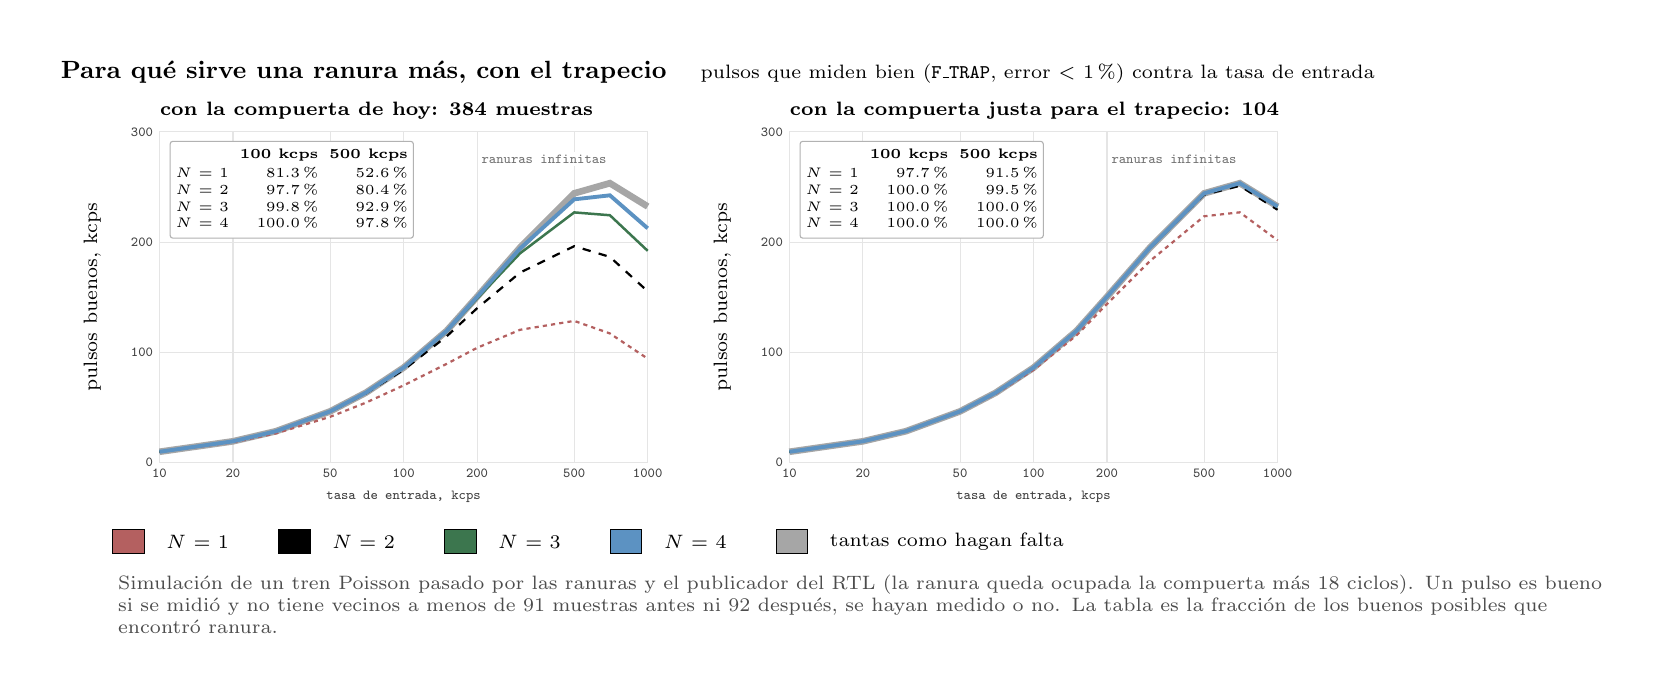
\begin{tikzpicture}[fondo]
\node[titulo] at (-1.4,5.25) {\textbf{Para qué sirve una ranura más, con el trapecio} \quad {\scriptsize pulsos que miden bien (\texttt{F\_TRAP}, error $<$ 1\,\%) contra la tasa de entrada}};
\node[anchor=south west, font=\scriptsize\bfseries, inner sep=0pt] at (0.000,4.350) {con la compuerta de hoy: 384 muestras};
\draw[black!50, line width=0.4pt] (0.000,0.000) rectangle (6.200,4.200);
\draw[black!10] (0.000,0.000) -- (6.200,0.000);
\node[nodo, anchor=east] at (-0.040,0.000) {0};
\draw[black!10] (0.000,1.400) -- (6.200,1.400);
\node[nodo, anchor=east] at (-0.040,1.400) {100};
\draw[black!10] (0.000,2.800) -- (6.200,2.800);
\node[nodo, anchor=east] at (-0.040,2.800) {200};
\draw[black!10] (0.000,4.200) -- (6.200,4.200);
\node[nodo, anchor=east] at (-0.040,4.200) {300};
\draw[black!10] (0.000,0.000) -- (0.000,4.200);
\node[nodo, anchor=north] at (0.000,-0.040) {10};
\draw[black!10] (0.933,0.000) -- (0.933,4.200);
\node[nodo, anchor=north] at (0.933,-0.040) {20};
\draw[black!10] (2.167,0.000) -- (2.167,4.200);
\node[nodo, anchor=north] at (2.167,-0.040) {50};
\draw[black!10] (3.100,0.000) -- (3.100,4.200);
\node[nodo, anchor=north] at (3.100,-0.040) {100};
\draw[black!10] (4.033,0.000) -- (4.033,4.200);
\node[nodo, anchor=north] at (4.033,-0.040) {200};
\draw[black!10] (5.267,0.000) -- (5.267,4.200);
\node[nodo, anchor=north] at (5.267,-0.040) {500};
\draw[black!10] (6.200,0.000) -- (6.200,4.200);
\node[nodo, anchor=north] at (6.200,-0.040) {1000};
\node[nodo, anchor=north] at (3.100,-0.320) {tasa de entrada, kcps};
\node[font=\scriptsize, anchor=south, rotate=90] at (-0.620,2.100) {pulsos buenos, kcps};
\draw[black!35, line width=2.4pt] plot coordinates {(0.000,0.138) (0.933,0.271) (1.479,0.399) (2.167,0.651) (2.620,0.888) (3.100,1.206) (3.646,1.673) (4.033,2.106) (4.579,2.731) (5.267,3.420) (5.720,3.549) (6.200,3.253)};
\node[nodo, anchor=east, text=black!55, fill=white, inner sep=1pt] at (5.720,3.857) {ranuras infinitas};
\draw[rojo!75!black, line width=0.8pt, dash pattern=on 1.5pt off 1.5pt] plot coordinates {(0.000,0.135) (0.933,0.258) (1.479,0.371) (2.167,0.582) (2.620,0.761) (3.100,0.981) (3.646,1.254) (4.033,1.458) (4.579,1.687) (5.267,1.800) (5.720,1.641) (6.200,1.320)};
\draw[black, line width=0.8pt, dashed] plot coordinates {(0.000,0.138) (0.933,0.271) (1.479,0.398) (2.167,0.647) (2.620,0.878) (3.100,1.179) (3.646,1.603) (4.033,1.960) (4.579,2.413) (5.267,2.749) (5.720,2.613) (6.200,2.176)};
\draw[verde!55!black, line width=0.9pt] plot coordinates {(0.000,0.138) (0.933,0.271) (1.479,0.399) (2.167,0.651) (2.620,0.887) (3.100,1.204) (3.646,1.664) (4.033,2.083) (4.579,2.658) (5.267,3.178) (5.720,3.142) (6.200,2.690)};
\draw[azul!85!black, line width=1.4pt] plot coordinates {(0.000,0.138) (0.933,0.271) (1.479,0.399) (2.167,0.651) (2.620,0.888) (3.100,1.206) (3.646,1.672) (4.033,2.104) (4.579,2.719) (5.267,3.344) (5.720,3.395) (6.200,2.976)};
\node[anchor=north west, font=\tiny, draw=black!30, fill=white, rounded corners=1pt, inner sep=2pt] at (0.128,4.088) {\begin{tabular}{@{}l@{\hspace{4pt}}r@{\hspace{4pt}}r@{}}& \textbf{100 kcps} & \textbf{500 kcps}\\[1pt]$N$ = 1 & 81.3\,\% & 52.6\,\%\\$N$ = 2 & 97.7\,\% & 80.4\,\%\\$N$ = 3 & 99.8\,\% & 92.9\,\%\\$N$ = 4 & 100.0\,\% & 97.8\,\%\\\end{tabular}};
\node[anchor=south west, font=\scriptsize\bfseries, inner sep=0pt] at (8.000,4.350) {con la compuerta justa para el trapecio: 104};
\draw[black!50, line width=0.4pt] (8.000,0.000) rectangle (14.200,4.200);
\draw[black!10] (8.000,0.000) -- (14.200,0.000);
\node[nodo, anchor=east] at (7.960,0.000) {0};
\draw[black!10] (8.000,1.400) -- (14.200,1.400);
\node[nodo, anchor=east] at (7.960,1.400) {100};
\draw[black!10] (8.000,2.800) -- (14.200,2.800);
\node[nodo, anchor=east] at (7.960,2.800) {200};
\draw[black!10] (8.000,4.200) -- (14.200,4.200);
\node[nodo, anchor=east] at (7.960,4.200) {300};
\draw[black!10] (8.000,0.000) -- (8.000,4.200);
\node[nodo, anchor=north] at (8.000,-0.040) {10};
\draw[black!10] (8.933,0.000) -- (8.933,4.200);
\node[nodo, anchor=north] at (8.933,-0.040) {20};
\draw[black!10] (10.167,0.000) -- (10.167,4.200);
\node[nodo, anchor=north] at (10.167,-0.040) {50};
\draw[black!10] (11.100,0.000) -- (11.100,4.200);
\node[nodo, anchor=north] at (11.100,-0.040) {100};
\draw[black!10] (12.033,0.000) -- (12.033,4.200);
\node[nodo, anchor=north] at (12.033,-0.040) {200};
\draw[black!10] (13.267,0.000) -- (13.267,4.200);
\node[nodo, anchor=north] at (13.267,-0.040) {500};
\draw[black!10] (14.200,0.000) -- (14.200,4.200);
\node[nodo, anchor=north] at (14.200,-0.040) {1000};
\node[nodo, anchor=north] at (11.100,-0.320) {tasa de entrada, kcps};
\node[font=\scriptsize, anchor=south, rotate=90] at (7.380,2.100) {pulsos buenos, kcps};
\draw[black!35, line width=2.4pt] plot coordinates {(8.000,0.138) (8.933,0.271) (9.479,0.399) (10.167,0.651) (10.620,0.888) (11.100,1.206) (11.646,1.673) (12.033,2.106) (12.579,2.731) (13.267,3.420) (13.720,3.549) (14.200,3.253)};
\node[nodo, anchor=east, text=black!55, fill=white, inner sep=1pt] at (13.720,3.857) {ranuras infinitas};
\draw[rojo!75!black, line width=0.8pt, dash pattern=on 1.5pt off 1.5pt] plot coordinates {(8.000,0.138) (8.933,0.270) (9.479,0.396) (10.167,0.643) (10.620,0.873) (11.100,1.178) (11.646,1.616) (12.033,2.015) (12.579,2.561) (13.267,3.129) (13.720,3.179) (14.200,2.823)};
\draw[black, line width=0.8pt, dashed] plot coordinates {(8.000,0.138) (8.933,0.271) (9.479,0.399) (10.167,0.651) (10.620,0.888) (11.100,1.206) (11.646,1.672) (12.033,2.104) (12.579,2.724) (13.267,3.403) (13.720,3.516) (14.200,3.211)};
\draw[verde!55!black, line width=0.9pt] plot coordinates {(8.000,0.138) (8.933,0.271) (9.479,0.399) (10.167,0.651) (10.620,0.888) (11.100,1.206) (11.646,1.673) (12.033,2.106) (12.579,2.731) (13.267,3.420) (13.720,3.548) (14.200,3.249)};
\draw[azul!85!black, line width=1.4pt] plot coordinates {(8.000,0.138) (8.933,0.271) (9.479,0.399) (10.167,0.651) (10.620,0.888) (11.100,1.206) (11.646,1.673) (12.033,2.106) (12.579,2.731) (13.267,3.420) (13.720,3.549) (14.200,3.253)};
\node[anchor=north west, font=\tiny, draw=black!30, fill=white, rounded corners=1pt, inner sep=2pt] at (8.128,4.088) {\begin{tabular}{@{}l@{\hspace{4pt}}r@{\hspace{4pt}}r@{}}& \textbf{100 kcps} & \textbf{500 kcps}\\[1pt]$N$ = 1 & 97.7\,\% & 91.5\,\%\\$N$ = 2 & 100.0\,\% & 99.5\,\%\\$N$ = 3 & 100.0\,\% & 100.0\,\%\\$N$ = 4 & 100.0\,\% & 100.0\,\%\\\end{tabular}};
\leyenda{-0.6,-1.0}{rojo!75!black/$N$ = 1, black/$N$ = 2, verde!55!black/$N$ = 3, azul!85!black/$N$ = 4, black!35/tantas como hagan falta}
  {Simulación de un tren Poisson pasado por las ranuras y el publicador del RTL (la ranura queda ocupada la compuerta más 18 ciclos). Un pulso es bueno si se midió y no tiene vecinos a menos de 91 muestras antes ni 92 después, se hayan medido o no. La tabla es la fracción de los buenos posibles que encontró ranura.}
\end{tikzpicture}
\end{document}
